Гравитационное линзирование -- явление отклонения траектории света от прямолинейной в гравитационном поле массивных объектов.  Это многогранное по своим свойствам и подробно описанное в литературе явление (см., например, \cite{gravlensbook}) является, в том числе, одним из независимых способов измерения ряда космологических констант, в частности, постоянной Хаббла $H_0$, определяющей темп расширения Вселенной в современную эпоху. В этом разделе приведены основные понятия, связанные с описанием так называемого \textbf{сильного гравитационного линзирования}. 

\subsection{Измерение расстояний}

Различные определения расстояния, используемые в космологии, приведены, например, в \cite{distance_measures}. Здесь и далее для описания расстояний между объектами в системе источник -- линза -- наблюдатель используется понятие \textbf{расстояния углового диаметра} (angular diameter distance). Оно определяется по следующей формуле (см, напр., уравн. №№14,15 в \cite{distance_measures}):

\begin{equation}\label{ang_dia_dist}
D_{A}\left(z_{1}, z_{2}\right)=\frac{c}{1+z_{2}} \int_{z_{1}}^{z_{2}} \frac{d z}{H_{0} \sqrt{\Omega_{m}\left(1+z^{3}\right)+\Omega_{\Lambda}}},
\end{equation}
где $H_0=70$ (км/с)/МПк, $\Omega_m=0.3, \Omega_\Lambda=0.7$. Выбор этих параметров обусловлен рассмотрением здесь и далее модели \textit{плоской вселенной}.

\subsection{Гравитационно-линзированная система}

При помощи общей теории относительности нетрудно показать (см., напр., \cite{gl_all}), что в гравитационном поле массивного тела \textit{(линзы)} с ньютоновским потенциалом $\Phi$ угол отклонения светового луча, испущенного \textit{источником} и пришедшего к \textit{наблюдателю}, равен

\begin{equation}
\hat{\alpha}=\frac{2}{c^{2}} \int_{-\infty}^{+\infty} \vec{\nabla}_{\perp} \Phi \ \mathrm{d} z,
\end{equation}
где $z$ - координата вдоль невозмущённой траектории распространения света. При этом предполагается, что $\Phi/c^2 \ll 1$, что выполняется практически всегда: например, для скопления галактик  $|\Phi|/c^2 \sim 10^{-4} \ll 1$. Это же условие обеспечивает малость углов: при сильном линзировании углы отклонения света порядка угловых секунд. Из того, что $\Phi$ не зависит от массы тела, попавшего в гравитационное поле, следует, что все фотоны отклоняются на один и тот же угол. В этом смысле сильное гравитационное линзирование \textit{ахроматично}, то есть не зависит от длины волны. 
%Для точечной линзы $\Phi=-\frac{G M}{r}$, где $M$ - её масса, а значит, что углы отклонения массивом таких линз могут быть сложены по принципу суперпозиции. 

В реалистичных моделях линз, в которых масса, вызывающая линзирование, распределена трёхмерным образом, используется \textit{приближение плоских линз}. Это всегда оправдано: характерные размеры самого большого объекта, который может быть линзой, - скопления галактик - порядка 1 МПк, в то время как типичное расстояние между объектами системы порядка 100-1000 МПк.
Типичная гравитационно-линзированная система изображена на Рисунке \ref{fig:gravlensfig}. Положения источника света и его изображения задаются углами, отсчитываемыми от \textit{оптической оси} - линии, проведённой от наблюдателя перпендикулярно плоскости линзы.

\begin{figure}[H]
    \centering
	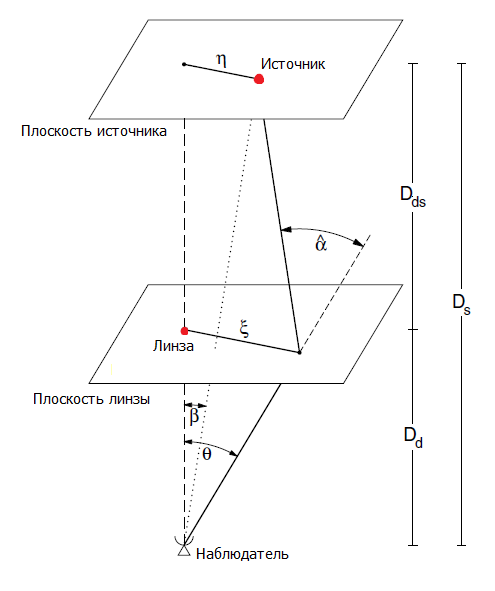
\includegraphics[scale=1.0]{pics/gravlenssyst.png}
	\caption{Типичная гравитационно-линзированная система (\cite{gravlensbook}). Здесь $\beta$ и $\theta$ - углы между оптической осью (пунктирная линия) и источником и его изображением соответственно, $\hat{\alpha}$ - угол отклонения светового луча, $\eta$ и $\xi$ - расстояния от оптической оси до источника и его изображения соответственно,  $D_d$ - расстояние между наблюдателем и плоскостью линзы, $D_{ds}$ - между плоскостями линзы и источника, $D_s$ - между наблюдателем и источником.\label{fig:gravlensfig} }
   \end{figure} 

Пусть масса линзы распределена в пространстве по закону $\rho(\overline \xi, z)$, где $\overline \xi$ - двумерный вектор в плоскости линзы, $z$ - координата вдоль оптической оси. \textit{Поверхностная плотность} линзы задаётся следующим соотношением:

\begin{equation}\label{sigmasurf}
\Sigma(\overline{\xi})=\int \rho(\vec{\xi}, z) \mathrm{d} z
\end{equation}

Характерным значением поверхностной плотности для линзы массой $M$ является \textit{критическая поверхностная плотность}:

\begin{equation}\label{sigmacrit}
\Sigma_{crit}=\frac{c^{2}}{4 \pi G} \frac{D_{\mathrm{s}}}{D_{\mathrm{d}} D_{\mathrm{ds}}},
\end{equation}
где $c$ - скорость света, $G$ - гравитационная постоянная, $D_d$, $D_s$ и $D_{ds}$ - расстояния от наблюдателя до плоскости линзы, до источника и между плоскостями линзы и источника соответственно (см. Рис. \ref{fig:gravlensfig}).

Радиус такой окружности в плоскости линзы, плотность внутри которой равна критической, называется \textit{радиусом Эйнштейна}. Обычно он выражается в угловых единицах: 

\begin{equation}\label{r_ein}
\theta_{E}=\sqrt{\frac{4 G M}{c^{2}} \frac{D_{d s}}{D_{d} D_{s}}}
\end{equation}

Также введём понятие безразмерной поверхностной плотности \textit{(convergence)}:
\begin{equation}\label{convergence}
\kappa = \frac{\Sigma}{\Sigma_{crit}}
\end{equation}
Такая запись удобна при разделении линзирующей массы на тёмную и барионную материю. В последнюю, в том числе, входят и отдельные звёзды, линзирование на которых исследуется в следующей главе. В дальнейшем безразмерная плотность звёзд будет обозначаться как $\kappa_*$, тёмной материи -- как $\kappa_c$.

\subsection{Усиление и искажение изображений}

С точки зрения линейной алгебры, гравитационное линзирование - это отображение плоскости источника на плоскость линзы, которое задаётся следующей матрицей:

\begin{equation}
\mathcal{A}(\boldsymbol{\theta})=\frac{\partial \boldsymbol{\beta}}{\partial \boldsymbol{\theta}}=\left(\delta_{i j}-\frac{\partial^{2} \psi(\boldsymbol{\theta})}{\partial \theta_{i} \partial \theta_{j}}\right)=\left(\begin{array}{cc}{1-\kappa-\gamma_{1}} & {-\gamma_{2}} \\ {-\gamma_{2}} & {1-\kappa+\gamma_{1}}\end{array}\right)
\end{equation}

В ней есть две основные составляющие: $\kappa$, отвечающая за изменение линейных размеров изображения (увеличение или уменьшение), и двухкомпонентный сдвиг \textit{(shear)} $\gamma=(\gamma_1,\gamma_2)$, характеризующий искажение формы изображений. Усиление изображения обратно пропорционально определителю этой матрицы (то есть якобиану этого отображения):
\begin{equation}
\mu=\frac{1}{\operatorname{det} A}
\end{equation}

Видно, что возможно существование некоторого множества точек, в которых усиление формально бесконечно. Кривая, образуемая этими точками, называется каустикой, а её образ в плоскости линзы – критической кривой. На Рисунке 2 видно, как ведёт себя изображение источника при пересечении им складки (fold) или излома (cusp) каустики.
 
\begin{figure}[H]
    \centering
	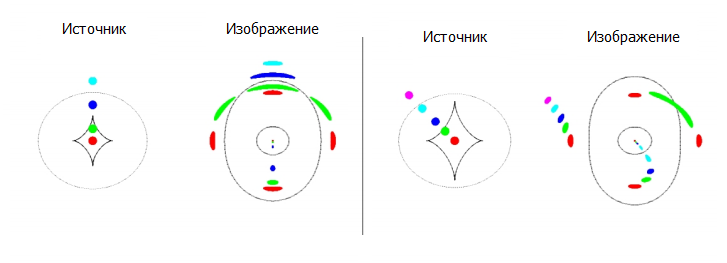
\includegraphics[scale=0.8]{pics/caust_intro.png}
	\caption{Поведение изображения (в плоскости линзы) источника при пересечении им излома (слева) или складки (справа) каустики  (\cite{narbart}). Также для иллюстрации изменения масштабов изображения нарисованы критические кривые в плоскости линзы}
\end{figure}

\subsection{Появление нескольких изображений}

Важным свойством гравитационного линзирования является возможность появления нескольких изображений одного и того же источника. В присутствии линзы существует дополнительная временная задержка между временем излучения света и моментом его прихода к наблюдателю по сравнению с прямолинейным приходом света:

\begin{equation}\label{tau}
\tau(\boldsymbol{\theta})=\frac{D_{d} D_{s}}{c D_{d s}}\left[\frac{1}{2}(\boldsymbol{\theta}-\boldsymbol{\beta})^{2}-\Psi(\boldsymbol{\theta})\right]
\end{equation}

Здесь первое слагаемое означает геометрическую задержку (удлиняется траектория распространения света), второе - гравитационную (в соответствии с ОТО время около гравитирующих тел идет “медленнее”); $\boldsymbol{\theta}$ и $\boldsymbol{\beta}$ -- положения (в угловых единицах) соответственно изображения и источника (см. Рис.\ref{fig:gravlensfig}), $\Psi(\boldsymbol{\theta})$ - линзирующий гравитационный потенциал. В соотвтетствии с принципом Ферма изображения формируются там, где $\nabla \tau = 0$. Следовательно, возможно появление нескольких изображений одного и того же источника (более подробное описание этого присутствует в \cite{gravlensbook}, \cite{gl_all}).

Так как оба слагаемых в формуле \eqref{tau} пропорциональны $H_0^{-1}$, то, измеряя временную задержку между изображениями одного и того же источника, можно получить значение постоянной Хаббла $H_0$. Идея использования именно линзированные сверхновые для оценки постоянной Хаббла была впервые предложена Сьюром Рефсдалом в 1964 году (\cite{refsdal1964}).

\section{Подходящие источники: квазары и сверхновые}

Для измерений временной задержки блеск источника должен быть переменным. В таком случае разные изображения, возникающие в результате гравитационного линзирования, будут изменять свой блеск также, как и источник, но с некоторой задержкой по времени. В качестве возможных источников для таких измерений используются квазары - они весьма яркие и почти точечные. На текущий момент опубликовано большое количество работ, посвящённых гравитационно линзированным квазарам и измерению при их помощи постоянной Хаббла (см, напр., работу \cite{holicow}, а также ссылки в ней). 

Другим подходящим источником являются сверхновые - их кривые блеска имеют чётко выраженный пик, а наблюдения занимают сравнительно небольшие времена, что значительно упрощает измерения. На текущий момент известны только две гравитационно линзированные сверхновые со множественными изображениями, SN Refsdal\footnote{Названа в честь Сьюра Рефсдала.} (\cite{kelly2014}) и SN iPTF16geu (\cite{goobar2017}). Однако с запуском в ближайшее время обсерватории LSST ожидается открытие десятков таких систем (\cite{pierelrodney2019}), что делает задачу разработки алгоритма анализа гравитационно линзированных сверхновых важной и своевременной.

